\section{What is an interactive meaningful experience?}

To be able to answer how one can design interactive meaningful experiences in a museum space that addresses sustainability, I will first have to explain what I mean when I talk about an interactive meaningful experience. In this section I will present research on sense-making in HCI, on how to support user’s active indexing in museums. This is the basis for understanding how visitors orient and understand, makes-sense-of, their surroundings and comprehend how fx. an installation is to be used. It can also in some way help us understand the relationship between attention span and engagement (as in sense-making being a pre-necessity to be able to meaning-making), how long time does the visitor spend in front of the installation before it gives up on it, because they cannot make sense of it. (bcz they dont understand it).

Eva Hornecker contributes to design/ hci knowledge on design for human agency, sense making, and mindful engagement with our environment. She present two conceptual notions; spatio-contextual embedding and indexing. These concepts serves and can be applied both in conceptual, analytical and in evaluating stages in the design process, and from the following article Hornecker presents 8 design strategies for the creation of spatio-contextual embedding and support of indexing. I intend to take with me these 8 design strategies in my synthesising of a framework to help design meaningful interactive museum experiences, where the strategies can be utilised in beginning or evaluative phases to aid in designing an interactive meaningful installation or experience.

\section{Meaning-making vs sense-making}
The two terms are similar, but in this thesis they have slightly different “functions” and is relevant in different “order”. The term sense-making is primarily used to describe and look at how someone makes sense of something. In a museum space - do they understand how something is to be used? When interacting with an interactive exhibition or installation, how intuitive is it to be used, and how long do people interact with it to “get it”. And is it clear why the installation is relevant in the museum space?

Meaning-making on the other hand is more than anything related to the reflective aspects of how something is made-sense of. It is more concerned with how the installation experience can give or take away reflections linked to the expository agency. As a designer one have to ask, or be able to answer, “what is it that this installation shall convey?” - and then look at how the interactive experience support that agency, in terms of the visitors reflections and after-thoughts somewhat align with it.

\section{The concept of Spatio-contextual embedding}
this is 100 direct quotation from article ::::::::: Based on case studies from a museum context, Hornecker present and illustrate the notion of “spatio-contextual embedding”, which conceptualises installation designs that augment real objects and environments while keeping primary focus on attention. Key for this “embeddedness” is that interaction is contextualised within a meaningful setting, creating relationships between system and environment. While retaining a focus on original objects or environments, it supports user’s active engagement and sense making by inviting, enticing, or forcing them to draw connections. At the heart of this is indexing. ::::::::::::: (Hornecker, p. 1)

The key takeaway is that design that is spatially contextualised and physically embedded, seem to engender and support indexing actions, and as a result of that increases the visitors engagement with its surroundings.


\section{The concept of Indexing}
There has been increased interest in the field of visitor studies and museum research in the details of visitor behaviour in museums, which is what the research done on indexing contributes to. (Hornecker, p. ??)

Hornecker’s working definition of indexing is explained as the mindful referencing back-and-forth between two representations or entities, comparing and relating them to each other and creating new meaning while doing so (Hornecker, p. 2). In the preface of the article we are presented to a story where a group of people are situated on a field trip to a hilltop, where the group make use of a panel with a simplified depiction of the view to make sense of and engage with the scenery. One of them point out a famous mountain on the panel, and then, points in the distance, saying its name, while the rest of them attempt to follow his reference. This is used as a simple example of what Hornecker refers to as the act of indexing.

Indexing practises support human sense-making and engages people with their surroundings (Hornecker, p. 39). Think of it as the mental process that happens when one tries to read the room, understand how something works, or how something is intended to be used. Indexing is the subtile interpretation act that manifests as sense-making. It is a useful concept for the interaction designer working in a museum or a similar exhibition domain, as a way to guide the design and evaluation of whether or not installations ‘makes sense’ for the visitor. It can be a helpful concept in terms of designing for the extension of time spent in front of/with the installation, and for rethinking the ‘unpopular’ installations, strengthening the exhibition experience as a whole.

Hornecker’s understanding of indexing is closer to the tradition of gesture studies and ethnography, which focus on the ways people coordinate their actions, in contrast to the semiotic tradition where the focus lies in the indexical sign’s ability to project or provide the visitor with the information needed to understand the context. Indexical expression are ubiquitous in our lives and an elementary part of our communication and coordination practises, as shown by conversation and ethnographic studies (Hornecker, p. 3). This linguistic-communicative understanding of indexing as suggested by Hornecker, is extended to include the notion of “indexing for yourself”, inspired by ideas which highlight how, for example, pointing can serve as a memory aid for individual cognition, using the external environment as a resource to aid cognition (Hornecker, p. 3). Which is why Hornecker’s notion of indexing is more positioned to expand the idea that people actively index to make connections between different things - that indexing is linked to the human action, not being a semiotic property of the artefact (Hornecker, p.5). Hornecker’s focus lies in identifying and understanding the user’s active indexing actions and in-detail investigation that takes place in the given situation, while investigating how technology explicitly can support and foster indexing (Hornecker, p. 2).


\section{Strategies for Creation of Spatio-Contextual Embedding and Support of Indexing
}
A new issue emerging from the studies presented in Hornecker’s article is how to design for indexicality. This means more than just integrating systems into a context, it is about purposely enabling users to make comparisons and references in both directions (Hornecker, p. 34). The strategies are translated into a question format, as this can make conceptual work more accessible for designers who dislike the vocabulary of design rules and guidelines, preferring open phrasing(Hornecker, p. 34), and the focus is on what to achieve rather than to avoid (Hornecker, p. 34). All of the strategies go together to create “contextual embedding”, however considerations and trade-offs need to be considered when combining strategies that fits your project or domain. (Hornecker, p. 34).

I intend to use the strategies in conceptual stages of prototyping. As well for evaluation/ analysis of installations and museum visits I have conducted. And, like I said in the beginning of this chapter, I intend to take with me these 8 design strategies in the synthesising of the framework that can help design meaningful interactive museum experiences. 

Hornecker presents this table with eight strategies for the creation of spatio-contextual embedding and the support of indexing;

\begin{figure}[H]
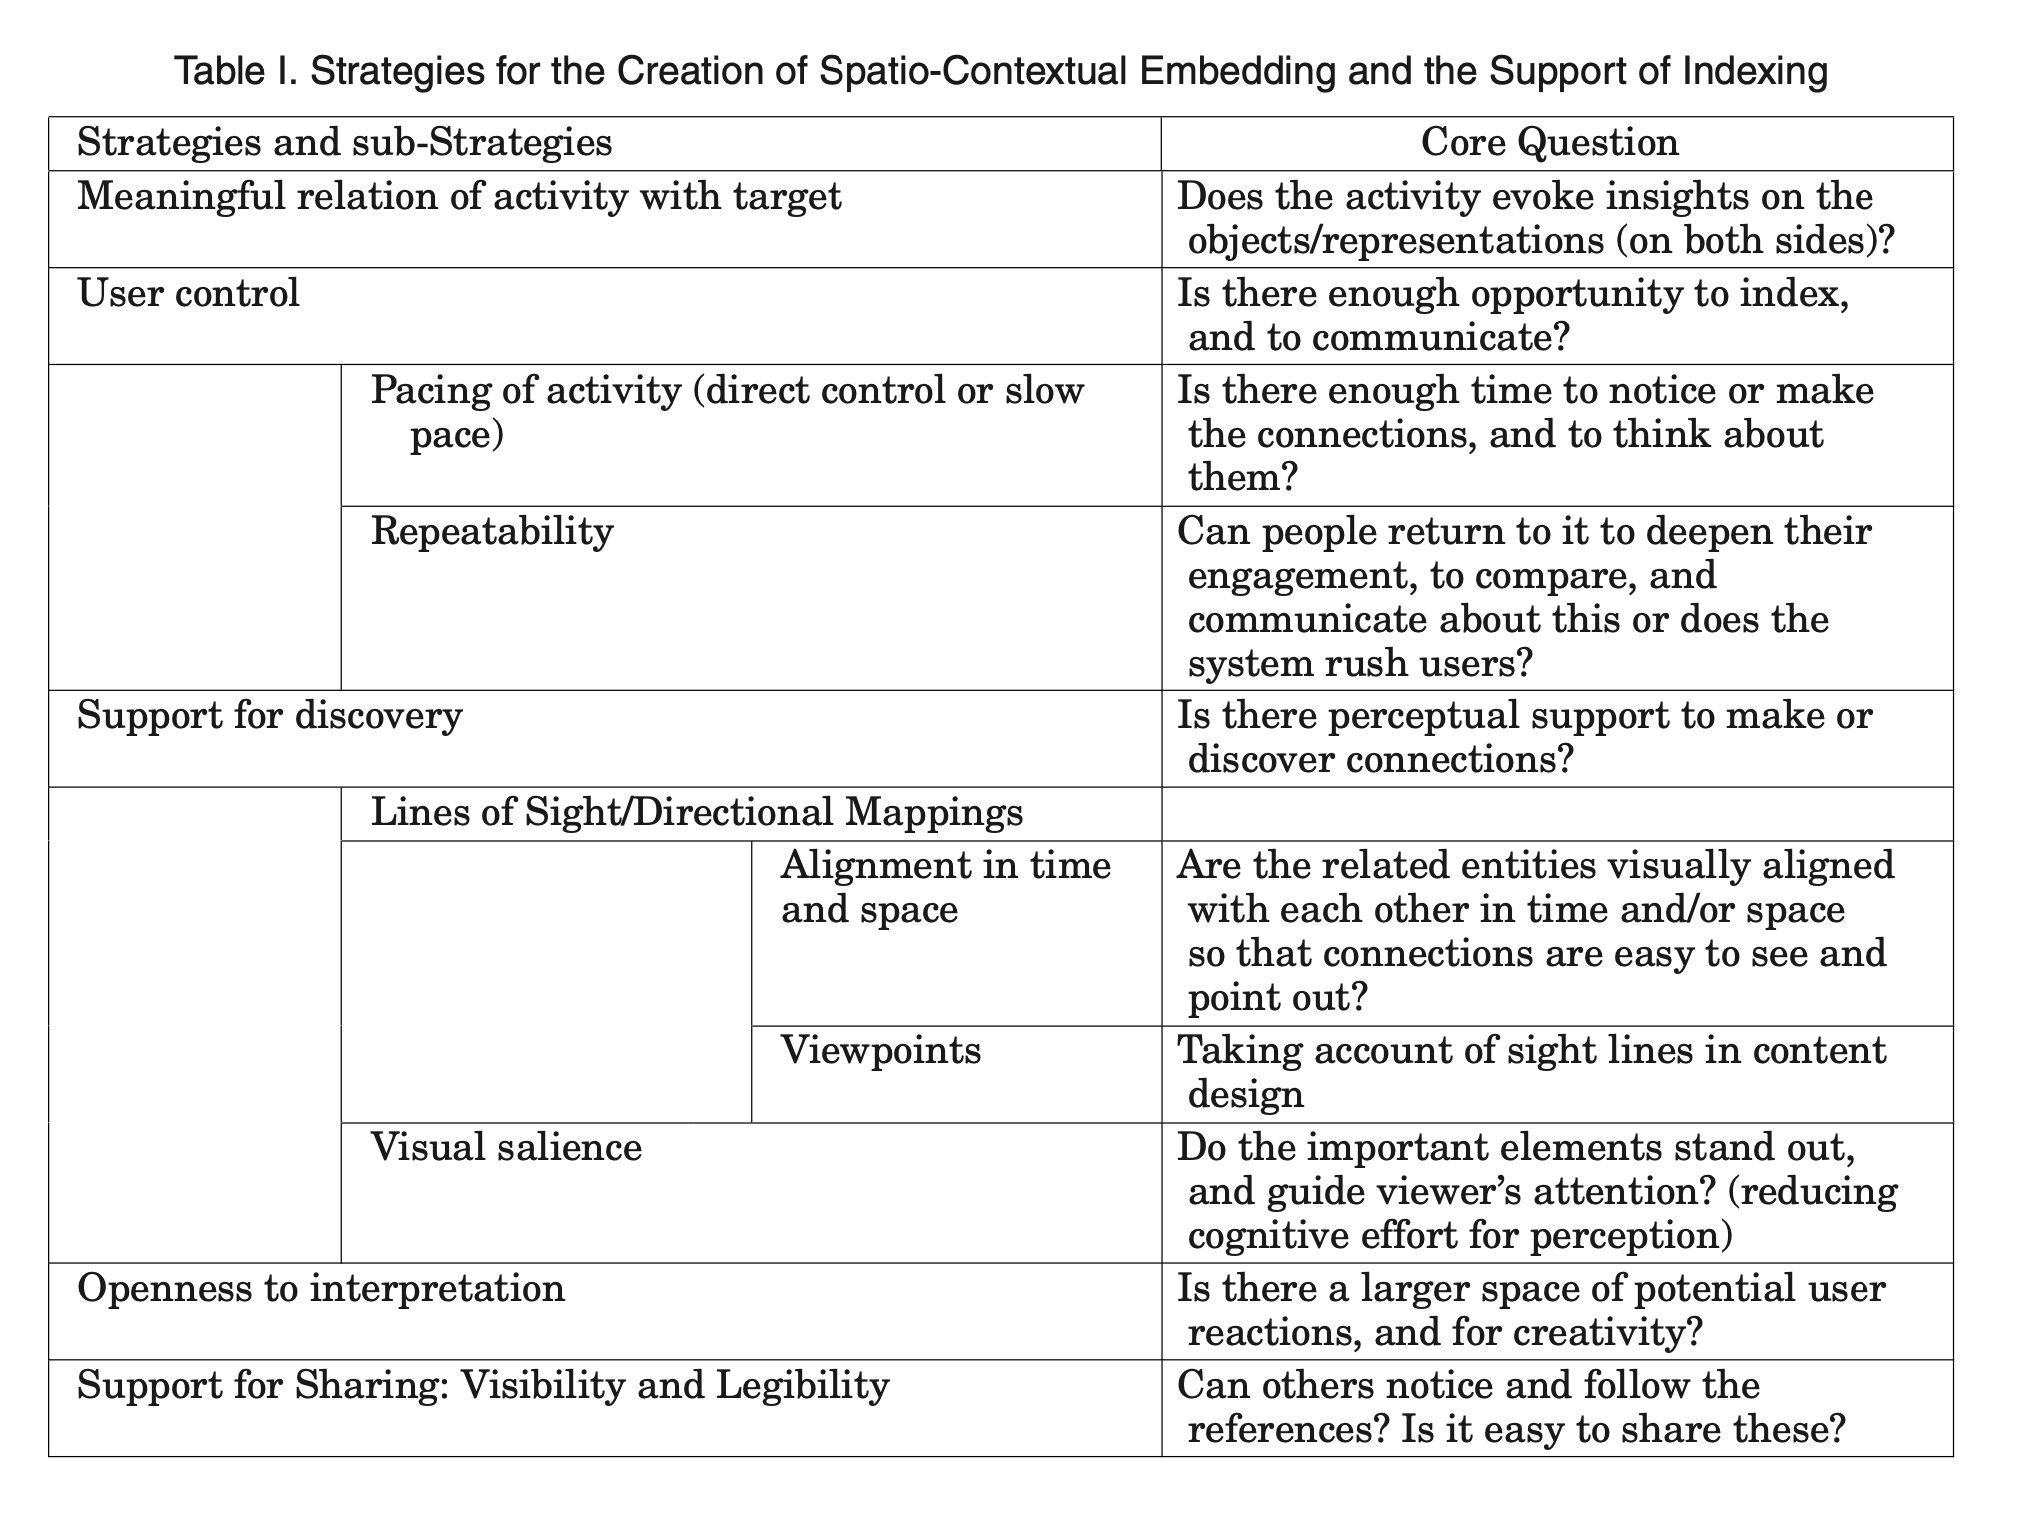
\includegraphics[width=12cm]{pictures/strategies.png}
\centering 
\end{figure}